\section{BIBDs and Examples}

Recall \Cref{lec1:defn-bibd}, the definition for Balanced Incomplete Block Designs (BIBD).

The \ul{parameters} ($v, b, r, k, \lambda$) of a BIBD are defined as follows:
\begin{itemize}
    \item $v = |V|$ - The number of points
    \item $b = |\B|$ - The number of blocks (also $\lambda_0$)
    \item $r = \lambda_1$ - Each point lies in $r$ blocks
    \item $k = |\alpha|, \forall \alpha \in \B$ - The size of the blocks
    \item $\lambda = \lambda_2$ - Each pair of points are in $\lambda$ blocks
\end{itemize}

We call $v, k, \lambda$ the \ul{primary} parameters and $b, r$ the \ul{secondary} parameters.

We'll call a BIBD with these parameters a:
\begin{itemize}
    \item $(v, k, \lambda)$-BIBD, or
    \item 2-$(v, k, \lambda)$-BIBD, or
    \item $(v, b, r, k, \lambda)$-BIBD
\end{itemize}

\begin{example}
    The Fano Plane (\Cref{lec1:exmp-fano-plane}) is a $(7,3,1)$-BIBD (and also a $(7,7,3,3,1)$-BIBD)
\end{example}

A BIBD is \ul{trivial} if $k \in \{0, 1, v-1, v\}$

\ul{Convention}: We will assume that our BIBDs are non-trivial designs (Since otherwise some statements \textit{may} be false)

\begin{definition}
    Let $(V, \B)$ be a design, we define the \ul{complement design} $(V, \overline{\B})$ where $\overline{\B} = \{V \setminus \alpha \:|\: \alpha \in \B \}$ 
\end{definition}

\begin{example}[Complement of the Fano Plane]
    ~\\
    $V = \{0, 1, 2, \ldots, 6\}$ - The points stay the same.

    $\B = \{013, 124, 235, 346, 450, 561, 602 \}$ - These were the blocks we had before.

    $\overline{\B} = \{2456, 0356, 0146, 0125, 1236, 0234, 1345 \}$ - These make a $(7, 7, 4, 4, 2)$-BIBD
\end{example}

\begin{exercise}
    The complement of a $(v, b, r, k, \lambda)$-BIBD is a $(v, b, b-r, v-k, b-2r+\lambda)$-BIBD
\end{exercise}

\subsection{Difference Sets}
Let $(G, +, 0)$ be an abelian group.
A difference set $S$ is a subset of $G$ with the property that there exists a constant $\lambda$ such that $\forall g \neq 0, \left\lvert\{(a,b) \in S \times S \:|\: a - b = g \}\right\rvert = \lambda$.
If $|G| = v, |S| = k$, we call this a $(v,k,\lambda)$-difference set

\begin{example}
    Let $G = \Z_7, S = \{0,1,3\}$.
    We can check that this is a difference set by taking the difference between every pair of elements $(a, b) \in S \times S$
    
    \begin{center}        
        \begin{tabular}{rc|c|c|c}
            \multicolumn{2}{c}{} & \multicolumn{3}{c}{a} \\
            & & 0 & 1 & 3 \\
            \cline{2-5}
            \multirow{3}{*}{b} & 0 & 0 & 1 & 3 \\
            \cline{2-5}
            & 1 & 6 & 0 & 2 \\
            \cline{2-5}
            & 3 & 4 & 5 & 0 \\
        \end{tabular}
    \end{center}

    Each number from 1 to 6 appear exactly once, so this is a $(7,3,1)$-difference set.
\end{example}

\begin{example}
    Let $G = \Z_{11}, S = \{0,2,3,4,8\}$ creates an (11,5,2)-difference set.
\end{example}

\begin{theorem}
    If $S \subseteq G$ is a $(v, k, \lambda)$-difference set, then we construct a $(v, k, \lambda)$-BIBD as follows:
    \begin{itemize}
        \item $V = G$
        \item $\B = \{g + S \:|\: s \in S \}$
    \end{itemize}
\end{theorem}
\begin{note}
    $v = b$ and $k = r$
\end{note}
\begin{proof}
    Exercise!
\end{proof}

\ul{Problem}: How to we find difference sets?
We'll see later in the course!

\subsection{Affine Space}
Let $V$ be a vector space over a finite field $\F$.
An affine line in $V$ is a set of points of the form $\setb{xt + y}{t \in \F}$, where $x, y \in V$, $x \neq 0$.
Let $\B$ be the set of all affine lines in $V$, then $(V, \B)$ is a BIBD with $\lambda = 1, k = |\F|$

When $\dim_\F V = 2$, we call this an \ul{affine plane}.

\begin{example}
    Let $\F = \Z_3, V = \Z_3^2$.
    This creates a $(9, 12, 4, 3, 1)$-BIBD.

    \begin{minipage}{\textwidth}
        \centering
        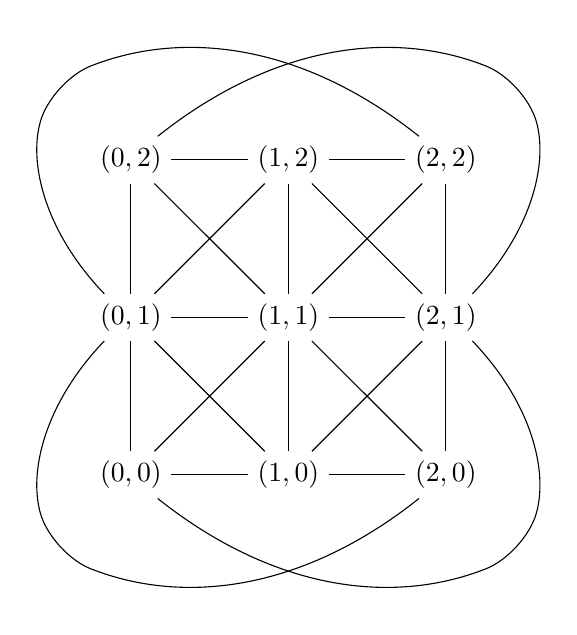
\begin{tikzpicture}
            \node (00) at (0,0) {$(0, 0)$};
            \node (01) at (0,2) {$(0, 1)$};
            \node (02) at (0,4) {$(0, 2)$};
            \node (10) at (2,0) {$(1, 0)$};
            \node (11) at (2,2) {$(1, 1)$};
            \node (12) at (2,4) {$(1, 2)$};
            \node (20) at (4,0) {$(2, 0)$};
            \node (21) at (4,2) {$(2, 1)$};
            \node (22) at (4,4) {$(2, 2)$};

            \draw (00) -- (11) -- (22);
            \draw (02) -- (11) -- (20);
            \draw (00) -- (01) -- (02);
            \draw (02) -- (12) -- (22);
            \draw (00) -- (10) -- (20);
            \draw (20) -- (21) -- (22);
            \draw (01) -- (11) -- (21);
            \draw (10) -- (11) -- (12);

            \draw[rounded corners = 15pt] (12) to (01) to[bend right] (-1, -1) to[bend right] (20); 
            \draw[rounded corners = 15pt] (10) to (21) to[bend right] (5, 5) to[bend right] (02); 
            \draw[rounded corners = 15pt] (12) to (21) to[bend left] (5, -1) to[bend left] (00); 
            \draw[rounded corners = 15pt] (10) to (01) to[bend left] (-1, 5) to[bend left] (22); 
        \end{tikzpicture}
    \end{minipage}

    For example, with $y = (1, 0), x = (2, 1)$, we have:
    \begin{itemize}
        \item $(1, 0) = 0x + y$
        \item $(0, 1) = 1x + y$
        \item $(2, 2) = 2x + y$
    \end{itemize}
    all of which are located on the same line.
\end{example}

\begin{example}
    The game of Set is a 4-dimensional affine space over $Z_3$
\end{example}

\subsection{Relations between Parameters}
\begin{theorem}
    The parameters $(v, b, r, k, \lambda)$ of a BIBD satisfy:
    \begin{align}
        \frac{v}{k} = \frac{b}{r} \\
        \frac{v(v-1)}{k(k-1)} = \frac{b}{\lambda} \\
        \frac{v-1}{k-1} = \frac{r}{\lambda}
    \end{align}
\end{theorem}
